\section{The Weekplanner Application}\label{sec:TheWeekplannerApplication}

The report document a lot of work on the Weekplanner application. The following section describes the key elements of the Weekplanner so it is easier to follow the nature of the work.

\subsection{Purpose}
Many people with an \gls{asd} need structure to function. Some \glspl{citizen} need visual presentation\cite{VisualSupport} of their schema because of limited verbal communication skills for example. 

There is a broad range of visual support tools for representing the schemas. One way is with the help of pictures. Each picture represent an activity.

\begin{figure}[H]
    \begin{center}
        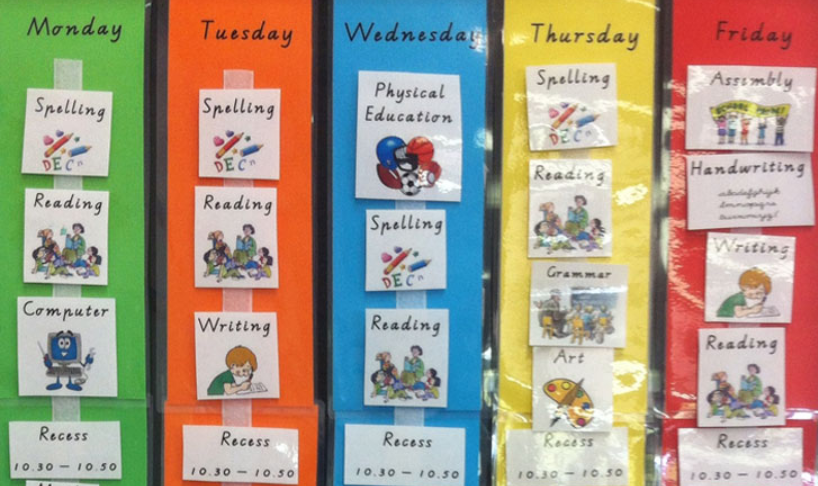
\includegraphics[width=0.95\textwidth]{figures/WeekPlanEks.png}
    \end{center}
    \caption{An example of a weekplan.\cite{VisualSupport}}
    \label{fig:WeekPlan}
\end{figure}

As illustrated on \autoref{fig:WeekPlan}, the activities is structured in days. Each day has a series of activities, and each activity is represented by a picture.
This is a common method of structuring activities but it has some problems. First it is inflexible. The schema cannot be moved around easily and the amount of activities cannot exceed the size of the board. Second, it is difficult to add new pictures and insert a picture in a day. 
The GIRAF costumers requested an application with the same functionality as the original tool, but more flexible to use and edit. This is the Weekplanner application. 

\subsection{Features}
There are two types of users, \gls{guardian} and \gls{citizen}. The schemas, called week plans, are connected to a \gls{citizen}. The \glspl{citizen} cannot log into the system. Guardians log into the system and get a list of citizens they are working with. When a \gls{citizen} is chosen all his week plans are shown, and a specific week plan can be chosen. 

The guardian can edit the week plan or change to citizen mode. In citizen mode the different activities can be marked as done, but a citizen cannot change the weekplan or navigate the application. From citizen mode, the system can be changed back to guardian mode.

The following describes only the screens that was implemented in the beginning of the semester. When this section was written we had changed the backend. This made it impossible to gain access to the original application, an we therefore have no screenshots of how et actually looked. Instead we have used the prototypes of the application to illustrate the pages.```

This ment that the application on Google Play could not login. It was not possible to build the application later, so we could not get pictures of the actual application. The pictures in this section is from the prototypes made by \gls{POT}.


The screens are:
\begin{itemize}
    \item Login
    \item Select citizen 
    \item Select Weekplan 
    \item Weekplan
    \item Find Pictogram
\end{itemize}

Here follows descriptions of each screen. The pictures are prototypes made for the costumers by \gls{POT}. 

\subsubsection*{Login Screen}
The login screen is similar to a standard login screen. The prototype can be seen in \ref{fig:LoginProt}

\begin{figure}[H]
    \begin{center}
        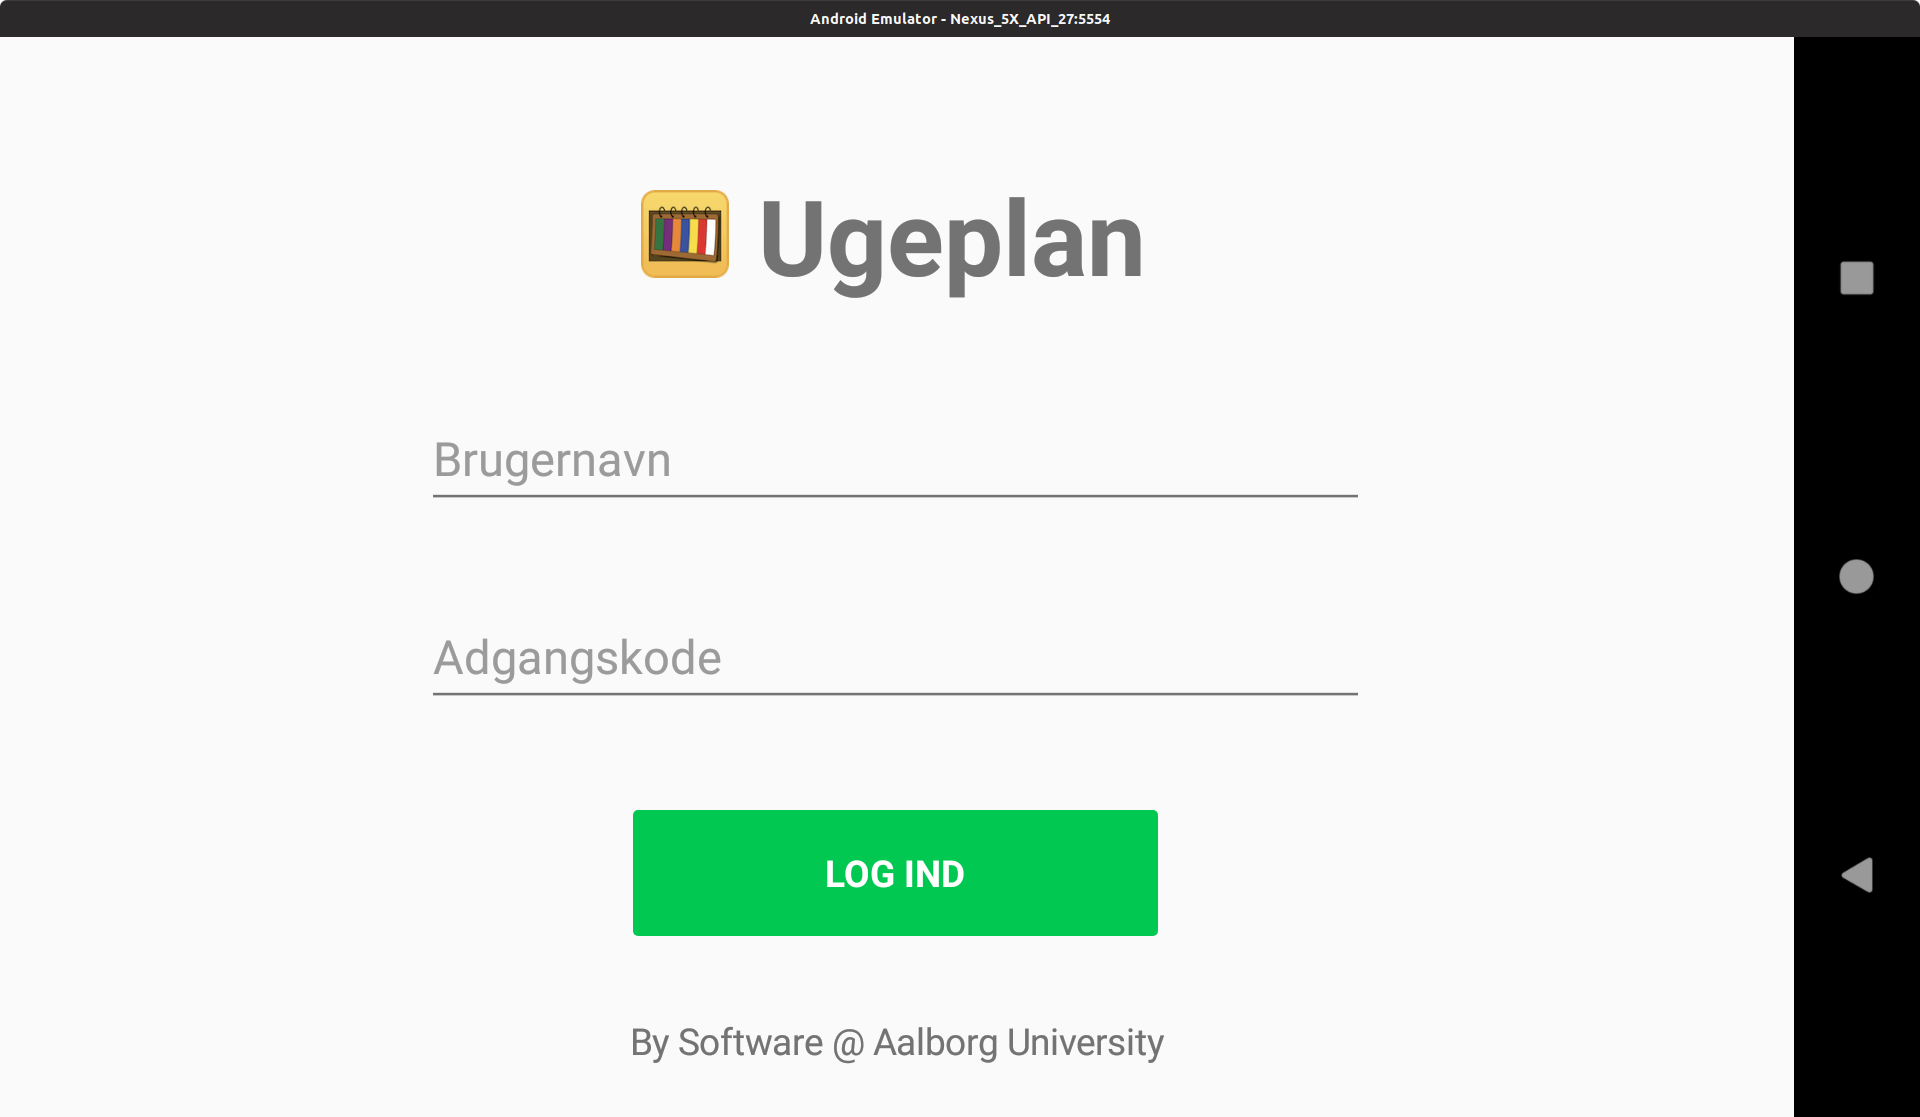
\includegraphics[width=0.95\textwidth]{figures/Prototypes/LoginScreenPrototype.png}
    \end{center}
    \caption{The prototype for the login screen}
    \label{fig:LoginProt}
\end{figure}
The application navigates to the Select Citizen screen after login. 

\subsubsection*{Select citizen screen}
The select citizen screen is shown in \ref{fig:ChooseCitProt}

\begin{figure}[H]
    \begin{center}
        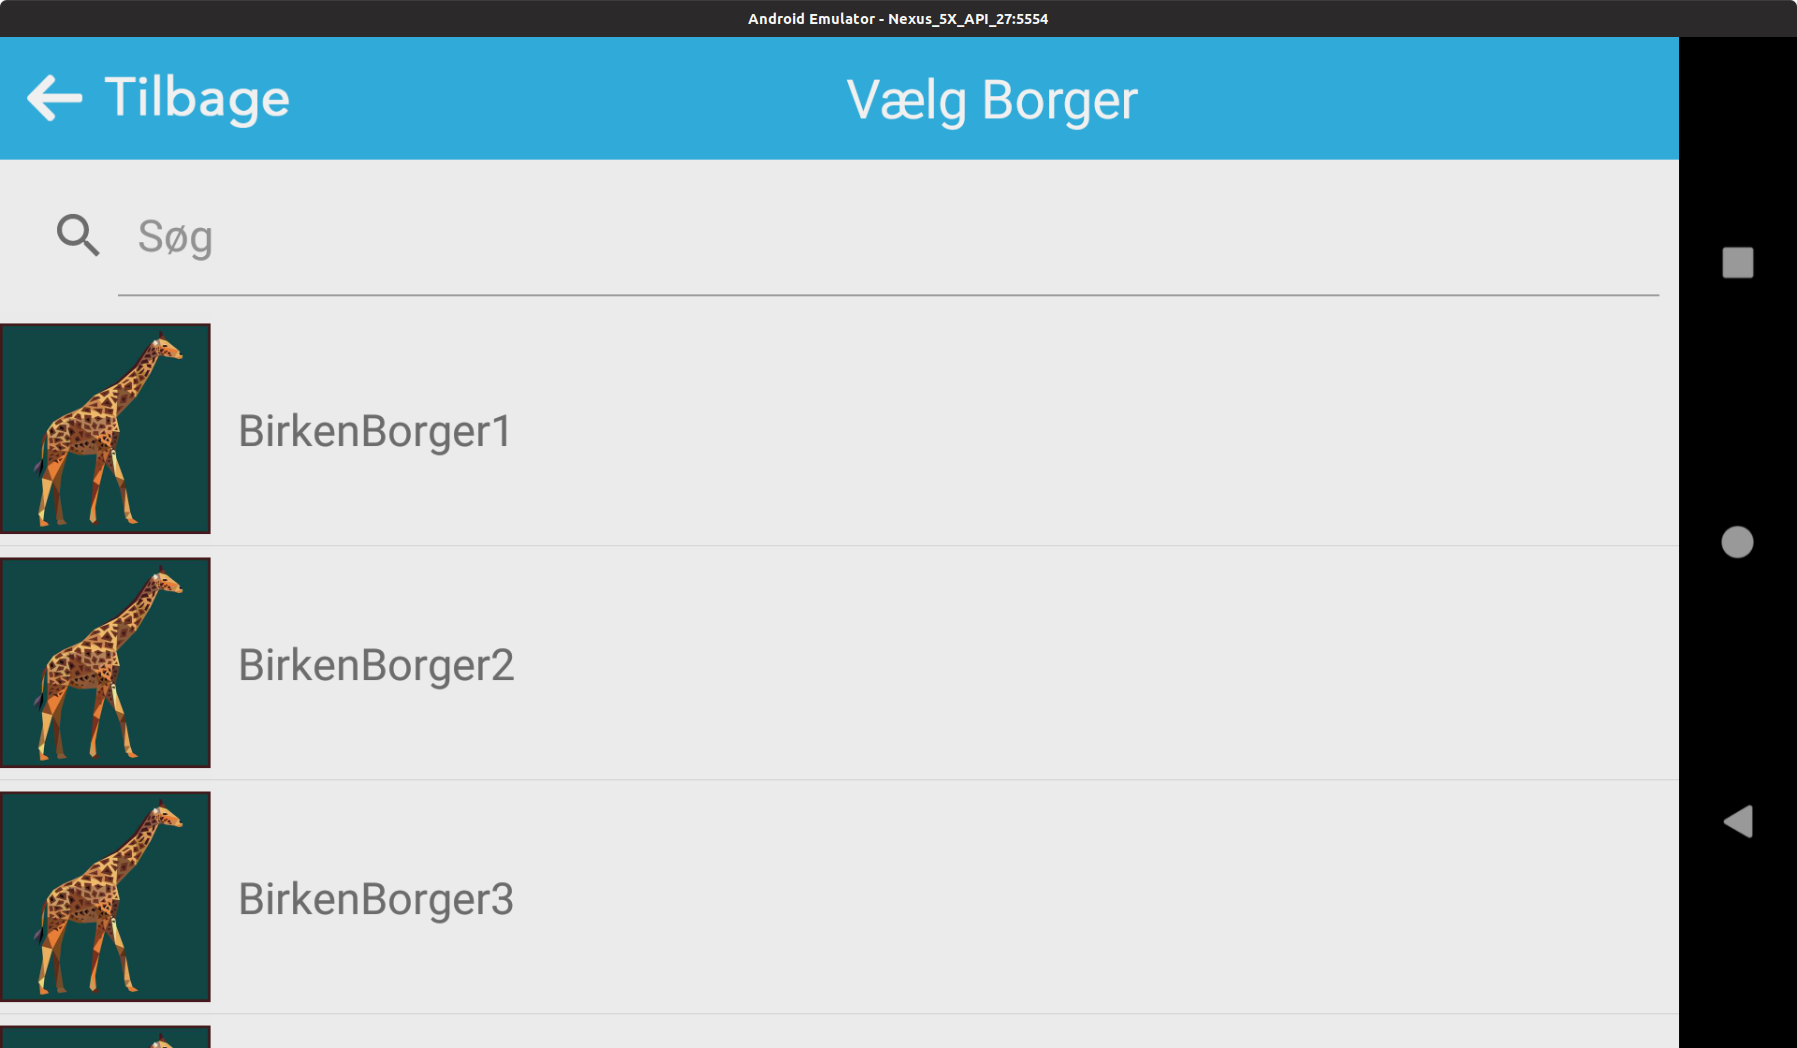
\includegraphics[width=0.95\textwidth]{figures/Prototypes/ChooseCitizenPrototype.png}
    \end{center}
    \caption{The prototype for the select citizen screen}
    \label{fig:ChooseCitProt}
\end{figure}

Here the guardian get a list of every citizen connected to him. The guardian can click on a citizen and then be directed to the Select Weekplan screen. 

\subsection*{Select Weekplan Screen}

\ref{fig:ChooseWeekProt} shows how the choose weekplan screen should look.
\begin{figure}[H]
    \begin{center}
        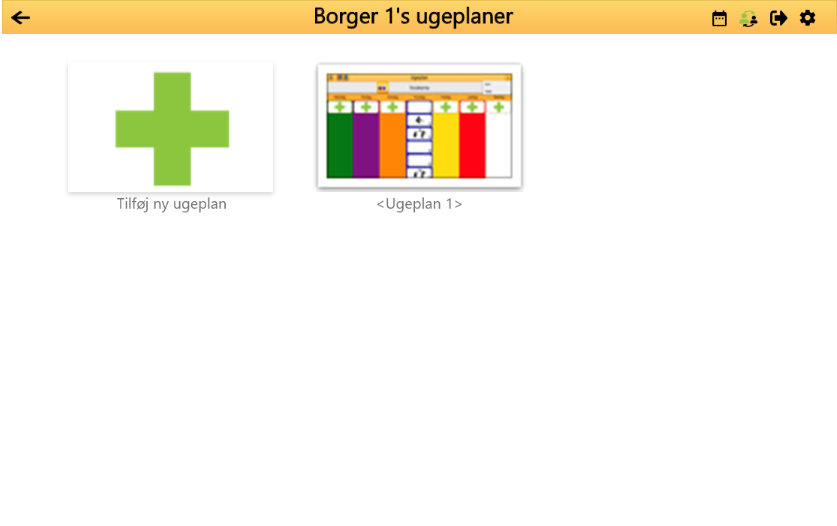
\includegraphics[width=0.95\textwidth]{figures/Prototypes/SelectWeekplanPrototype.png}
    \end{center}
    \caption{The prototype for the select weekplan screen}
    \label{fig:ChooseWeekProt}
\end{figure}

For each weekplan connected to the choosen citizen, a picture of the weekplan with it's name is shown. There is also a button for adding a new weekplan to the citizen.
The guardian is directed to the weekplan screen after choosing a plan.

\subsection*{Weekplan Screen}
There are two types of weekplan screens, the citizen screen, \ref{fig:WeekplanCitProt}, and the guardian screen, \ref{fig:WeekplanGuarProt}. 

%De to kunne måske være side om side??
\begin{figure}[H]
    \begin{center}
        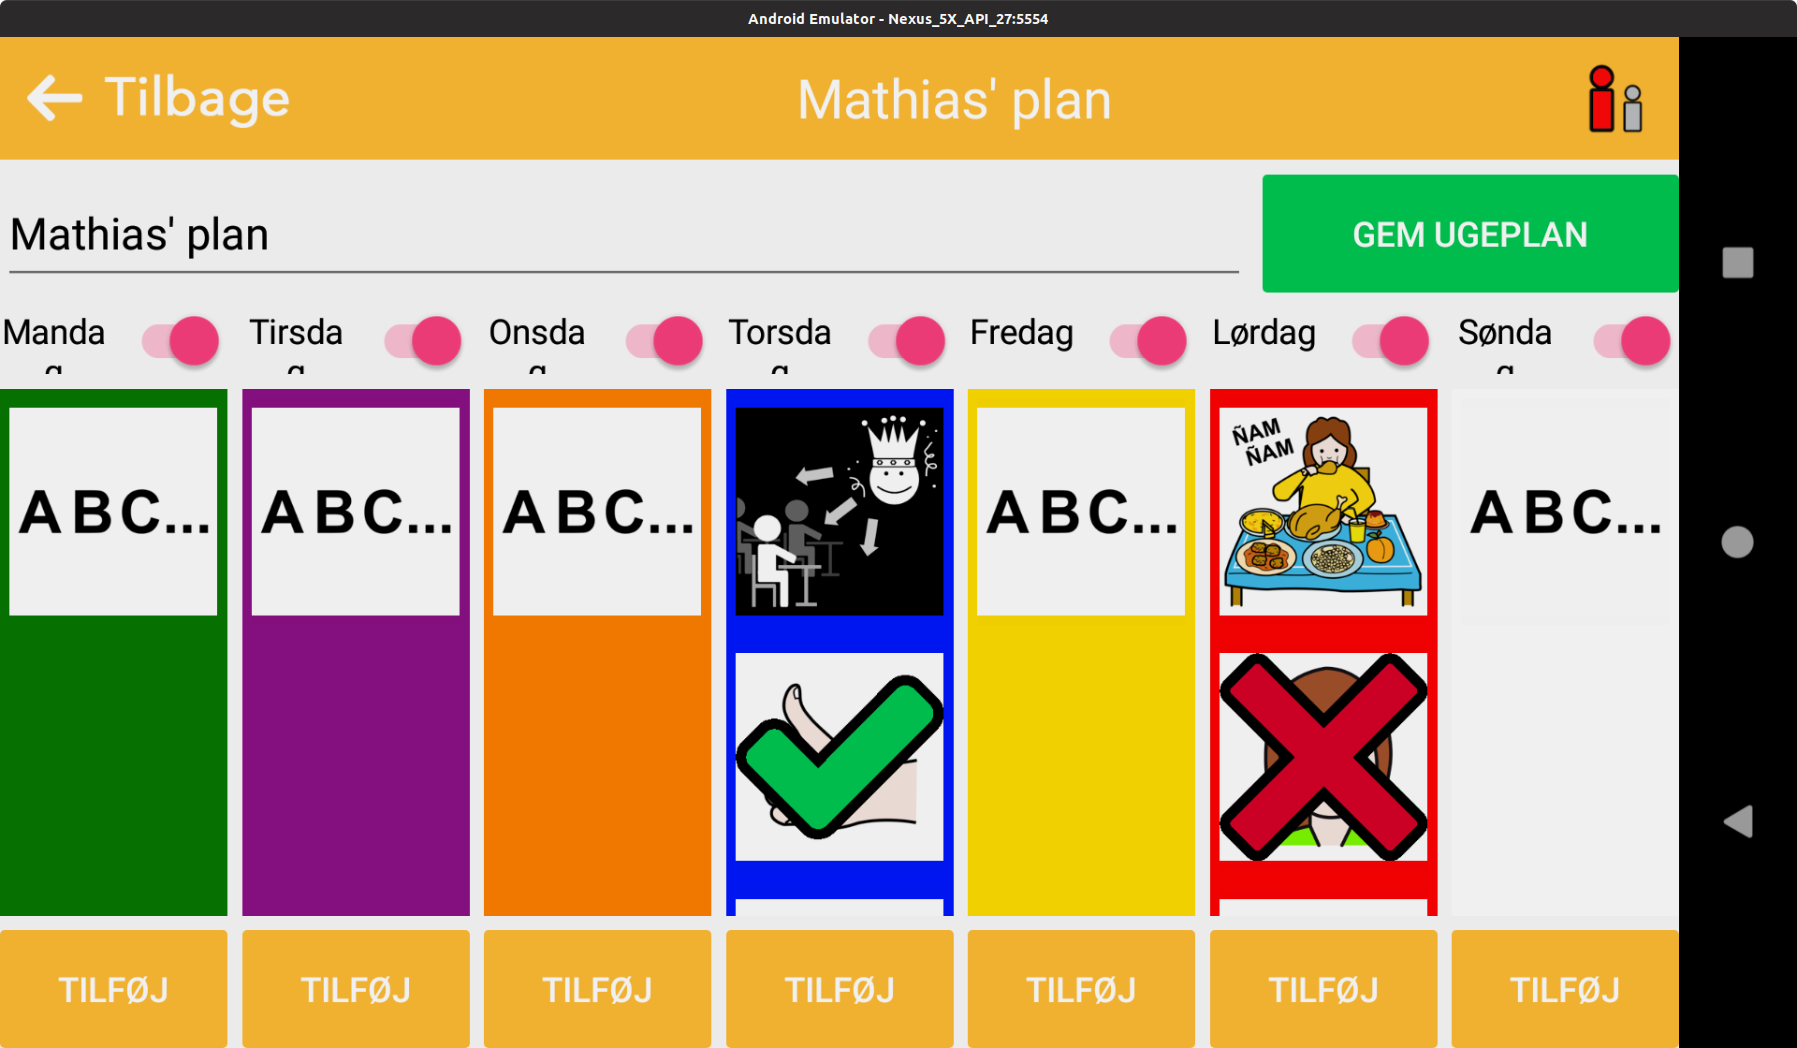
\includegraphics[width=0.95\textwidth]{figures/Prototypes/WeekPlannerGuardianPrototype.png}
    \end{center}
    \caption{The guardian version of the weekplan screen}
    \label{fig:WeekplanGuarProt}
\end{figure}

\begin{figure}[H]
    \begin{center}
        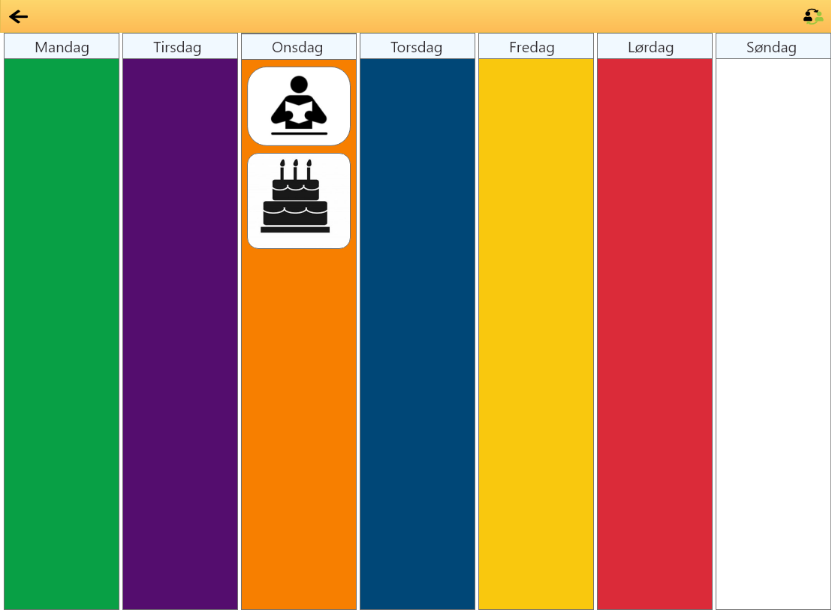
\includegraphics[width=0.95\textwidth]{figures/Prototypes/WeekPlannerCitizenPrototype.png}
    \end{center}
    \caption{The citizen version of the weekplan screen}
    \label{fig:WeekplanCitProt}
\end{figure}

In both screens you can see the activities planned for the day, but when an activity is clicked on, on the citizen screen, they are marked as done, while they can be edited on the guardian screen. The guardian screen is also the only screen where you can add activities.

The features working on the start of the semester is the following:
\begin{itemize}
    \item Login 
    \item Choose citizen 
    \item Choose weekplan
    \item Mark activity as done 
    \item Add activity
    \item Remove activity
    \item Switch to guardian mode
\end{itemize}

Other features are planned for later development.
